%% 04_results.tex
% Numbers from: analysis/results.md, analysis/recall_at_k.md,
%               analysis/latency_tokens.md, analysis/feature_extraction.md,
%               analysis/error_taxonomy.md

\section{Results}
\label{sec:results}

\subsection{Overall Accuracy}
\label{sec:results:overall}

% Source: analysis/results.md, Section 1
Table~\ref{tab:main_results} reports overall exact-match accuracy for all three systems
on the 13,800-question evaluation (N per system, fully paired by question\_id).
System~A (Narrative RAG) achieves 40.6\% exact-match (Wilson 95\%~CI [39.8\%, 41.4\%]),
outperforming System~B (Structured Naive) at 35.3\% [34.5\%, 36.1\%] and System~C
(Structured Aware) at 33.4\% [32.6\%, 34.2\%].

\begin{table}[htbp]
\centering
\caption{Overall exact-match accuracy (N = 13,800 per system, fully paired).
Wilson 95\% CIs shown. Paired bootstrap differences and McNemar test statistics
are reported separately in Table~\ref{tab:pairwise}.}
\label{tab:main_results}
\begin{tabular}{lccc}
\toprule
System & Correct & Exact-match & Wilson 95\% CI \\
\midrule
A -- Narrative RAG & 5,600 & 40.6\% & [39.8\%, 41.4\%] \\
B -- Structured Naive & 4,873 & 35.3\% & [34.5\%, 36.1\%] \\
C -- Structured Aware & 4,605 & 33.4\% & [32.6\%, 34.2\%] \\
\bottomrule
\end{tabular}
\end{table}

% Source: analysis/results.md, Sections 2--3
All three pairwise differences are statistically significant.
Table~\ref{tab:pairwise} shows paired bootstrap confidence intervals and McNemar
test statistics; all bootstrap CIs exclude zero and all McNemar $p < 0.001$.

\begin{table}[htbp]
\centering
\caption{Pairwise accuracy comparisons. Paired bootstrap (10,000 resamples, seed 42,
paired by question\_id). McNemar $\chi^2$ uses the uncorrected formula $(b-c)^2 / (b+c)$
with 1~df, where $b$ is the count of questions where the first system is correct
and the second is wrong, and $c$ is the converse. Phi = effect size.}
\label{tab:pairwise}
\begin{tabular}{lcccc}
\toprule
Comparison & Observed diff (pp) & Bootstrap 95\% CI & Discordant ($b$, $c$) & McNemar $\chi^2$ ($p$, $\phi$) \\
\midrule
A vs.\ B & +5.27 & [+4.5\%, +6.0\%] & (1{,}792, 1{,}065) & 185.0 ($p{<}0.001$, $\phi{=}0.116$) \\
A vs.\ C & +7.21 & [+6.4\%, +8.0\%] & (1{,}994, 999) & 330.8 ($p{<}0.001$, $\phi{=}0.155$) \\
B vs.\ C & +1.94 & [+1.3\%, +2.5\%] & (1{,}027, 759) &  40.2 ($p{<}0.001$, $\phi{=}0.054$) \\
\bottomrule
\end{tabular}
\end{table}

The effect sizes (phi 0.054--0.155) are modest, consistent with a 5--7 percentage-point
absolute gap on a large, difficult question set.  By Cohen's convention the A vs.\ B
($\phi{=}0.116$) and A vs.\ C ($\phi{=}0.155$) effects sit between "very small" and "small";
the B vs.\ C effect ($\phi{=}0.054$) is below the conventional small-effect threshold.
The McNemar test detects the B vs.\ C gap as significant given the large sample size
(N=13,800), but the two structured systems are practically equivalent on this evaluation.
We return to their practical significance in Section~\ref{sec:discussion}.

\paragraph{Partial credit.}
The partial-credit metric (defined in \S\ref{sec:methods:eval}) tracks exact-match
closely overall: A 0.438, B 0.380, C 0.360.  The largest exact-to-partial gap appears on \texttt{temporal\_comparison}
(missed-dose detection), where System~A rises from 43.7\% exact to 58.3\% partial
($+14.6$~pp) and System~C from 34.3\% to 43.5\% ($+9.2$~pp).  This indicates that on
date-valued answers the systems often produce a date close to the ground truth but
outside the exact-match criterion; the partial-credit signal does not change the
A $>$ B $>$ C ordering.

\subsection{Complexity Gradient}
\label{sec:results:tiers}

\begin{figure}[!ht]
\centering
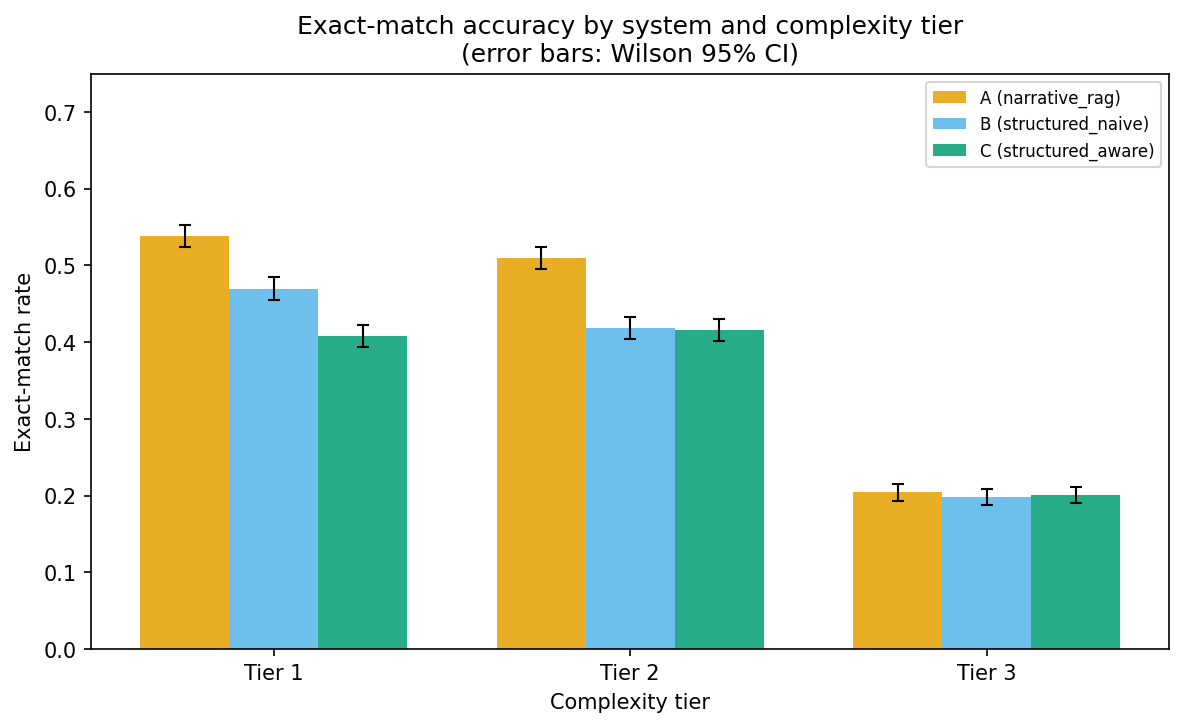
\includegraphics[width=0.85\textwidth]{../figures/accuracy_by_tier.png}
\caption{Exact-match accuracy by system and complexity tier (Wilson 95\% CI error bars).
Tier~1: single long-acting injectable; Tier~2: cyclic regimen; Tier~3: multi-drug.
All three systems converge near 20\% at Tier~3, with 95\%~CIs below the
within-family most-frequent-class baseline at 24.8\%; on Tier~3 multi-drug regimens
the systems perform worse than a trivial within-family majority predictor, and the
result is robust to a doubled (1024-token) output budget
(\S\ref{sec:results:budget_sweep}).}
\label{fig:accuracy_by_tier}
\end{figure}

% Source: analysis/results.md, Section 5
Figure~\ref{fig:accuracy_by_tier} plots accuracy by tier for all three systems.
A sharp complexity gradient is observed across all systems: Tier~1 accuracy is
approximately 41--54\% while Tier~3 collapses uniformly to approximately 20\% regardless
of retrieval architecture.

\begin{table}[htbp]
\centering
\caption{Accuracy by complexity tier (Wilson 95\% CIs).
Tier 1: single LAI on fixed schedule; Tier 2: cyclic regimen; Tier 3: multi-drug.
$n$ is the question count per tier (each patient contributes 69 questions).}
\label{tab:tier_results}
\small
\begin{tabular}{lccccc}
\toprule
Tier & $n$ (questions) & A & B & C \\
\midrule
1 & 4,347 & 53.9\% [52.4, 55.3] & 47.0\% [45.5, 48.5] & 40.8\% [39.3, 42.2] \\
2 & 4,347 & 51.0\% [49.5, 52.5] & 41.8\% [40.4, 43.3] & 41.6\% [40.2, 43.1] \\
3 & 5,106 & 20.4\% [19.3, 21.6] & 19.8\% [18.7, 20.9] & 20.1\% [19.0, 21.2] \\
\bottomrule
\end{tabular}\\[2pt]
\footnotesize Cells show exact-match accuracy with Wilson 95\% CI in brackets.
\end{table}

% Source: analysis/results.md, Section 5 monotonicity notes
Systems A and B show monotone decline (A: 53.9\% $>$ 51.0\% $>$ 20.4\%; B: 47.0\%
$>$ 41.8\% $>$ 19.8\%).  System~C shows a non-monotone pattern at Tiers~1--2
(40.8\% at Tier~1, 41.6\% at Tier~2), consistent with the resource-aware retriever
providing more benefit on cyclic multi-component questions than on simple single-LAI
lookups.

% Source: analysis/tier3_baseline.md (run_tier3_baseline.py)
At Tier 3 all three systems converge to $\approx 20\%$, but a per-family
most-frequent-class baseline (predict the modal ground-truth label within each
question family on Tier 3) reaches \textbf{24.8\% [23.6\%, 26.0\%]}.  The 95\%~CIs
of the three systems (A:~[19.3\%, 21.6\%]; B:~[18.7\%, 20.9\%]; C:~[19.0\%, 21.2\%])
sit below the baseline CI: every system is significantly worse than the
trivial within-family majority predictor on Tier~3 multi-drug regimens.  This
shifts the interpretation: at Tier 3 the answer LLM is not merely under-budgeted
on multi-step temporal reasoning, it is actively misled by retrieved context relative
to a constant prediction strategy.  We analyse the retrieval-vs-reasoning attribution
of this Tier-3 failure in Section~\ref{sec:discussion}, using a per-family Tier-3
recall@k breakdown that shows the retrieved context generally contains the supporting
evidence even on questions the systems answer incorrectly.

\subsection{By Question Family}
\label{sec:results:families}

% Source: analysis/results.md, Section 4
Table~\ref{tab:family_results} reports accuracy by question family.

\begin{table}[htbp]
\centering
\caption{Accuracy by PSP adherence-indicator family (Wilson 95\% CIs).
Family legend: \texttt{temporal\_lookup} = next-dose lookup;
\texttt{regimen\_aggregation} = dose-history aggregation (MPR numerator);
\texttt{regimen\_compliance} = coverage-window reasoning (PDC);
\texttt{temporal\_comparison} = missed-dose detection;
\texttt{cross\_resource} = persistence / cross-resource component questions.}
\label{tab:family_results}
\small
\begin{tabular}{lcccc}
\toprule
Family & $n$ & A & B & C \\
\midrule
\texttt{temporal\_lookup}     & 3,200 & 56.2\% [54.5, 57.9] & 49.0\% [47.3, 50.8] & 49.8\% [48.1, 51.6] \\
\texttt{temporal\_comparison} & 2,400 & 43.7\% [41.7, 45.7] & 43.7\% [41.7, 45.7] & 34.3\% [32.5, 36.3] \\
\texttt{cross\_resource}      & 1,600 & 43.4\% [41.0, 45.8] & 44.5\% [42.1, 46.9] & 43.4\% [41.0, 45.9] \\
\texttt{regimen\_compliance}  & 4,200 & 30.9\% [29.5, 32.3] & 25.6\% [24.3, 26.9] & 25.3\% [24.0, 26.6] \\
\texttt{regimen\_aggregation} & 2,400 & 31.8\% [30.0, 33.7] & 19.5\% [18.0, 21.1] & 17.8\% [16.4, 19.4] \\
\bottomrule
\end{tabular}\\[2pt]
\footnotesize Cells show exact-match accuracy with Wilson 95\% CI in brackets.
\end{table}

Two findings stand out.  The cross\_resource family is at parity across all three systems
(A=43.4\%, B=44.5\%, C=43.4\%), indicating that the advantage of structured or
resource-aware retrieval does not emerge on multi-resource relational questions at this
difficulty level, at least within the current answer budget.  The narrative advantage is
largest on regimen\_aggregation (A leads B by 12.3~pp; bootstrap CI excludes zero) and
regimen\_compliance (A leads B by 5.3~pp), reflecting that FHIR JSON serialisation
imposes a context-length cost that hurts dose-count arithmetic.

\subsection{Retrieval Recall vs.\ Answer Accuracy}
\label{sec:results:recall}

% Source: analysis/recall_at_k.md
System~A recall@k is N/A: narrative chunks carry no FHIR resource IDs and a
resource-level recall cannot be defined.  For Systems~B and~C, Table~\ref{tab:recall}
shows overall recall@5.

\begin{table}[htbp]
\centering
\caption{Retrieval recall@k (B vs.\ C). System~A = N/A (no FHIR resource IDs on
narrative chunks). Values shown as mean recall [Wilson 95\% CI mean across strata].}
\label{tab:recall}
\footnotesize
\begin{tabular}{lcccc}
\toprule
System & $k=1$ & $k=3$ & $k=5$ & $k=10$ \\
\midrule
B -- Structured Naive  & 0.573 [0.543, 0.602] & 0.739 [0.711, 0.765] & 0.762 [0.735, 0.787] & 0.762 [0.735, 0.787] \\
C -- Structured Aware  & 0.664 [0.636, 0.690] & 0.829 [0.807, 0.848] & 0.852 [0.831, 0.870] & 0.852 [0.831, 0.870] \\
\bottomrule
\end{tabular}
\end{table}

System~C retrieves the relevant resource more often than System~B at $k=1$ (0.664 vs.\
0.573) and $k=5$ (0.852 vs.\ 0.762).  The $k=1$ gap confirms that the resource-aware
primitives (typed filter, reference traversal, temporal pre-filter) correctly rank the
relevant resource higher.
However, this retrieval advantage \emph{does not translate into an end-to-end accuracy
advantage}: C scores 33.4\% exact-match vs.\ B's 35.3\%.  The most likely explanation
is that the FHIR-JSON context fed to the answer LLM remains harder to reason over
than narrative text, even when the correct resource is retrieved.

\subsection{Latency, Tokens, and Cost}
\label{sec:results:latency}

% Source: analysis/latency_tokens.md
Table~\ref{tab:latency} summarises latency and token usage.

\begin{table}[htbp]
\centering
\caption{Latency (milliseconds), mean token usage per call, and cost.
Cost estimated at Groq Developer-plan pricing (\$0.29/M tokens-in, \$0.59/M tokens-out).
Cost-per-correct = total cost divided by exact-match correct answers (5{,}600 / 4{,}873 /
4{,}605 for A / B / C respectively).}
\label{tab:latency}
\begin{tabular}{lcccccc}
\toprule
System & p50 (ms) & p95 (ms) & p99 (ms) & Tokens-in (mean) & Total cost (USD) & Cost / correct \\
\midrule
A -- Narrative  & 1,060 & 6,031  & 53,038 &   490 & \$4.74  & \$0.00085 \\
B -- Naive      & 1,354 & 17,890 & 46,301 & 4,463 & \$21.07 & \$0.00432 \\
C -- Aware      & 1,056 & 4,538  &  8,513 & 2,175 & \$6.88  & \$0.00149 \\
\bottomrule
\end{tabular}
\end{table}

System~B's 9$\times$ context expansion (4,463 vs.\ 490 mean tokens-in) drives a
4.4$\times$ cost premium over System~A on total spend (\$21.07 vs.\ \$4.74), but the
gap widens to roughly 5$\times$ on a cost-per-correct-answer basis (\$0.00432 vs.\
\$0.00085) because the extra spend buys fewer correct answers.  System~B also has
the highest tail latency (p99 = 46,301~ms).  System~C's resource-aware filtering
reduces context by $\approx$51\% vs.\ B, yielding the lowest p50 latency (1,056~ms)
and a 1.76$\times$ cost-per-correct premium over A (\$0.00149).  Neither structured
system is cost-effective relative to System~A given the accuracy deficit.

\subsection{Error Taxonomy}
\label{sec:results:errors}

% Source: analysis/error_taxonomy.md
\begin{figure}[!ht]
\centering
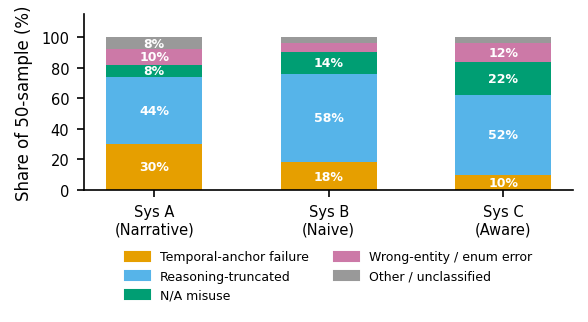
\includegraphics[width=0.85\textwidth]{../figures/error_taxonomy_distribution.png}
\caption{Error category distribution across the stratified failure sample
(n=50 per system, seed=42; colours: Wong colorblind-safe palette~\citep{wong2011points}).
Reasoning truncation (dark blue) is the single largest category for all three systems.
Temporal-anchor failures (orange) are highest for System~A, declining across B and C.}
\label{fig:error_taxonomy}
\end{figure}

Figure~\ref{fig:error_taxonomy} and Table~\ref{tab:errors} show the distribution of
failure modes across a stratified sample of 50 failures per system (10 per family, seed 42).

\begin{table}[htbp]
\centering
\caption{Error taxonomy distribution (n=50 per system, stratified by family).
Seed = 42. Single-rater classification by deterministic regex rules.}
\label{tab:errors}
\begin{tabular}{lcccccc}
\toprule
Category & A ($n$) & A (\%) & B ($n$) & B (\%) & C ($n$) & C (\%) \\
\midrule
Reasoning-truncated       & 22 & 44\% & 29 & 58\% & 26 & 52\% \\
Temporal-anchor failure   & 15 & 30\% & 9  & 18\% & 5  & 10\% \\
N/A misuse                & 4  & 8\%  & 7  & 14\% & 11 & 22\% \\
Wrong-entity / enum       & 5  & 10\% & 3  & 6\%  & 6  & 12\% \\
Other / unclassified      & 4  & 8\%  & 2  & 4\%  & 2  & 4\%  \\
\midrule
\textbf{Total}            & \textbf{50} & & \textbf{50} & & \textbf{50} & \\
\bottomrule
\end{tabular}
\end{table}

Reasoning truncation is the dominant failure mode across all three systems (44--58\%),
reflecting the 512-token output budget.  The rate is highest for B (58\%) and C (52\%)
because FHIR-JSON contexts require longer chain-of-thought arithmetic before a final answer
can be stated; the same LLM, given the same reasoning task, runs out of budget sooner when
the context is denser.  This is a token-budget artefact, not an architectural property of
narrative vs.\ structured retrieval.

Temporal-anchor failures follow a gradient: 30\% for A, 18\% for B, 10\% for C.
Narrative chunks do not embed the question's reference date (a per-question parameter, not
a feature of the narrative text), so the LLM must infer the temporal anchor from context.
FHIR resources (\path{CarePlan.period.start/end}, \path{MedicationAdministration.effectiveDateTime})
provide explicit date fields from which a temporal anchor can sometimes be inferred,
explaining the lower rate for B and C.

N/A misuse increases from A (8\%) to C (22\%): structured systems retrieve FHIR components
directly, making it more likely that the model encounters records for absent components
(Tier-1 patients have no adjunct or rescue component) and computes a phantom value rather
than returning N/A.

\subsection{Feature-Extraction Arm}
\label{sec:results:o6}

% Source: analysis/feature_extraction.md
Table~\ref{tab:auc} reports AUC-ROC for the synthetic adherence classification task
(label: $\geq$2 consecutive missed doses in final 60~d OR median gap $>$ 1.5$\times$
prescribed interval in final 90~d; class balance 14.5\% positive / 85.5\% negative;
200 patients; 5-fold stratified CV).

\begin{table}[htbp]
\centering
\caption{Feature-extraction arm AUC-ROC. Bootstrap 95\% CIs at patient level from
out-of-fold predictions (10,000 resamples). Both classifiers use
\texttt{class\_weight="balanced"} for parity (the original
preprint left LightGBM unweighted; we re-ran with class-weighting after peer review and
report the resulting numbers here; the unweighted numbers differ by under 0.03~AUC in
every cell and preserve the relative ordering).
FS-Structured = FHIR-derived numerics;
FS-Narrative = heuristic regex on LLM narratives; FS-Aware = per-patient aggregates
from System~C retrieval traces.}
\label{tab:auc}
\begin{tabular}{lcc}
\toprule
Feature set & LightGBM AUC & Logistic Regression AUC \\
\midrule
FS-Structured & 0.997 [0.983, 1.000] & 1.000 [0.999, 1.000] \\
FS-Narrative  & 0.846 [0.761, 0.889] & 0.836 [0.764, 0.897] \\
FS-Aware      & 0.769 [0.660, 0.844] & 0.708 [0.634, 0.799] \\
\bottomrule
\end{tabular}
\end{table}

% Source: analysis/feature_extraction.md, pairwise differences (class-weighted re-run)
Pairwise bootstrap differences (LightGBM, class-weighted):
FS-Structured vs.\ FS-Narrative $\Delta{=}+0.167$ [+0.104, +0.234];
FS-Structured vs.\ FS-Aware $\Delta{=}+0.238$ [+0.150, +0.336];
FS-Narrative vs.\ FS-Aware $\Delta{=}+0.071$ [$-0.039$, $+0.190$].
Reported $\Delta$ values are bootstrap means and may differ from the point-estimate
differences in Table~\ref{tab:auc} by approximately one percentage point due to
resampling variance.  The FS-Narrative vs.\ FS-Aware CI straddles zero: these two
feature sets are tied within the bootstrap interval.

% Source: analysis/feature_extraction.md, interpretation note
The near-perfect FS-Structured AUC (0.997--1.000) is partly a synthetic-data
artefact: the positive label is concentrated entirely in Tier-2 patients (all 29
positives are Tier~2; no Tier-1 or Tier-3 patient is labelled positive in this
perfectly-scheduled synthetic dataset).  FS-Structured features encode tier as one-hot
columns and directly capture the cyclic off-period gap via \texttt{gap\_max\_90d} and
\texttt{n\_events\_60d}.  FS-Narrative captures tier through ``tier~2'' / ``T2''
text patterns; FS-Aware captures it through the retrieval distribution.
The relative ordering (Structured $\gg$ Narrative $\approx$ Aware) and the CI widths
are genuine signals about information richness under these feature extraction strategies,
even if the absolute AUC values are inflated by the synthetic-label structure.
Readers should not extrapolate the FS-Structured ceiling to real-world noisy adherence
data.

\subsection{Output-Budget Sensitivity Sweep}
\label{sec:results:budget_sweep}

% Source: analysis/token_sweep_compare.md (run_token_sweep_compare.py).
% Sample: 33 questions per (tier x family) cell = 495 paired questions, seed 42.
The error taxonomy attributes 44--58\% of failures to reasoning truncation under the
512-token output budget (\S\ref{sec:results:errors}).  To test whether this artefact
is the cause of the A $>$ B $>$ C ordering, we re-ran all three systems on a stratified
495-question sample (33 per tier $\times$ family cell, seed~42) at
\texttt{ANSWER\_MAX\_TOKENS} = 1024.  Results are paired by question id and reported as
the bootstrap-mean delta (1024 minus 512) with 10,000-resample 95\%~CIs
(Table~\ref{tab:budget_sweep}).

\begin{table}[htbp]
\centering
\caption{Effect of doubling the answer-token budget from 512 to 1024 on the same 495
question ids.  Paired bootstrap (10,000 resamples, seed 42).  Sample-level 512-token
accuracies match the population-level estimates in Table~\ref{tab:main_results}
within sampling noise.}
\label{tab:budget_sweep}
\begin{tabular}{lccc}
\toprule
System & 512 acc & 1024 acc & Paired $\Delta$ (95\% CI) \\
\midrule
A -- Narrative RAG     & 44.2\% & 44.2\% & $+0.000$ [$-0.022$, $+0.022$] \\
B -- Structured Naive  & 35.2\% & 39.0\% & $+0.038$ [$+0.010$, $+0.067$] \\
C -- Structured Aware  & 33.1\% & 38.2\% & $+0.051$ [$+0.022$, $+0.081$] \\
\bottomrule
\end{tabular}
\end{table}

Three findings emerge.  First, System~A is unaffected by the larger budget (paired
$\Delta = 0.000$, CI straddling zero): no question changes its exact-match outcome
between 512 and 1024 tokens, even though 16\% of A's 1024-token answers exceed
512 tokens.  This is consistent with the narrative format not requiring long
chain-of-thought arithmetic to produce a final answer.

Second, both structured systems gain significantly: B by $+3.8$~pp [$+1.0$, $+6.7$]
and C by $+5.1$~pp [$+2.2$, $+8.1$].  C gains slightly more than B, narrowing the
B vs.\ C gap from $1.9$~pp at 512 tokens to $0.8$~pp at 1024 tokens.  The
A vs.\ C gap narrows from $7.2$~pp to $6.0$~pp.  The A $>$ B $>$ C ordering survives
at 1024 tokens; the budget effect partially closes but does not eliminate the gap.

Third, the Tier~3 collapse is robust to the budget.  At 1024 tokens, all three
systems still sit at $\approx$21\% on Tier~3 (paired tier-3 deltas: A $-0.6$~pp,
B $+1.2$~pp, C $+1.2$~pp; all CIs straddle zero).  The structured-system gains
concentrate on Tier~1 and Tier~2 (e.g.\ C Tier-1 $+7.3$~pp [$+1.8$, $+13.3$];
B Tier-2 $+6.1$~pp [$+0.0$, $+12.1$]).  The Tier~3 multi-drug failure described in
\S\ref{sec:results:tiers} is therefore not a budget artefact and remains an open
problem.  By family, the largest structured-system gains land on
\texttt{temporal\_lookup} (B $+9.1$~pp; C $+12.1$~pp) and \texttt{regimen\_compliance}
(B $+9.1$~pp; C $+10.1$~pp); \texttt{cross\_resource} and \texttt{regimen\_aggregation}
do not gain, consistent with the cross-resource scope statement in
\S\ref{sec:discussion}.

\subsection{No-Retrieval Baseline}
\label{sec:results:noretrieval}

% Source: results/scored_noretrieval/scored.csv (run via scripts/run_no_retrieval_arm.py)
To decompose absolute accuracy into a question-text-attributable component and a
retrieval-attributable component, we run a fourth arm (System~N) that passes each
question to the answer LLM with empty retrieved context.  All other variables --
answer LLM, system prompt, temperature, max\_tokens -- are identical to A/B/C.
With no patient context, qwen3-32b answers from question-text priors alone, giving a
floor for what the model can guess about specialty-medication adherence without any
patient-specific evidence.

System~N achieves $25.2\%$~[$24.4\%$, $25.9\%$] exact-match on the full
13{,}800-question evaluation, lifting roughly two-thirds of System~A's absolute
accuracy and three-quarters of Systems~B and~C's.  Per-tier the picture is sharper:
no-retrieval accuracy is $35.1\%$ at Tier~1, $36.7\%$ at Tier~2, and collapses to
$6.9\%$~[$6.2\%$, $7.6\%$] at Tier~3 -- well below both the per-family modal
baseline (24.8\%) and every retrieval system (19.8--20.4\%).

Paired bootstrap differences (system minus no-retrieval; 10{,}000 resamples; seed
42) confirm that retrieval contributes real signal in every comparison:
A vs.\ N $\Delta{=}{+}15.4$~pp $[+14.6$, $+16.3]$;
B vs.\ N $\Delta{=}{+}10.1$~pp $[+9.3$, $+11.0]$;
C vs.\ N $\Delta{=}{+}8.2$~pp $[+7.3$, $+9.1]$.  All CIs exclude zero.  The
relative ordering of retrieval-attributable accuracy (A $>$ B $>$ C) matches the
overall accuracy ordering, so the A advantage on QA is not driven by a higher
question-text-attributable floor: the gap between A and the structured systems
comes from how much each retrieval substrate adds to the question-text prior.

Three caveats.  First, at Tier~3 retrieval contributes a roughly uniform $+13$~pp
across A, B, and C, but the resulting accuracy ($\approx{20}\%$) still sits below
the modal baseline (24.8\%).  The interpretation in \S\ref{sec:results:tiers}
that the systems are ``actively misled by retrieved context relative to a constant
prediction strategy'' is consistent with this: retrieval is doing real work on
Tier~3, just not enough work to overcome the LLM's confused reasoning on
multi-component regimens.  Second, by family the no-retrieval baseline is highest
on \texttt{regimen\_compliance} ($34.9\%$) and \texttt{temporal\_lookup} ($33.1\%$),
indicating that those families contain a high fraction of questions whose modal
answer is guessable from text (yes/no or canonical dosing-interval responses); the
retrieval-attributable lift on those families is correspondingly smaller.  The
\texttt{regimen\_aggregation} family has the lowest no-retrieval baseline ($5.3\%$),
matching the intuition that arithmetic over administration events is essentially
ungiessable without the underlying data.  Third, this decomposition holds A/B/C's
shared answer LLM and prompt template constant; it does not address whether a
different answer LLM with weaker priors would shift the floor.

\begin{table}[htbp]
\centering
\caption{No-retrieval baseline (System~N) and retrieval-attributable accuracy per
system.  Retrieval-attributable = paired exact-match accuracy difference vs.\
System~N on the same 13{,}800 questions; 95\% CIs from 10{,}000-resample paired
bootstrap, seed 42.}
\label{tab:noretrieval}
\begin{tabular}{lccc}
\toprule
System & Overall accuracy & Retrieval-attributable (pp) & 95\% CI \\
\midrule
N -- No retrieval & 25.2\% & --- & --- \\
A -- Narrative   & 40.6\% & $+15.4$ & $[+14.6, +16.3]$ \\
B -- Naive       & 35.3\% & $+10.1$ & $[+9.3, +11.0]$ \\
C -- Aware       & 33.4\% & $+8.2$  & $[+7.3, +9.1]$ \\
\bottomrule
\end{tabular}
\end{table}

\subsection{Templated-Narrative Ablation: Is the A Advantage LLM-Specific?}
\label{sec:results:templated}

% Source: results/scored_templated/scored.csv and analysis/templated_compare.md
% (run via scripts/run_templated_arm.py + analysis/run_templated_compare.py)
The headline finding that System~A wins QA leaves an attribution question
unresolved: does narrative \emph{format} drive the advantage, or do
LLM-generated narratives carry additional structure (lexical regularity,
idiomatic clinical phrasing) beyond format alone?  To disambiguate, we ran a
fifth arm (System A-T) in which the canonical System~A pipeline -- same
chunker, same BGE embedder, same retriever, same answer LLM, same
ANSWER\_MAX\_TOKENS, same answer prompt template -- is pointed at the
deterministic templated narratives instead of the LLM-generated narratives.
Both narrative sources passed the same prompted-entity fidelity audit at
100\% recall (\S\ref{sec:methods:dataset}).  Only the narrative text differs
between A and A-T.

A-T achieves $41.3\%$~[$40.5\%$, $42.1\%$] exact-match accuracy, compared to
A's $40.6\%$~[$39.8\%$, $41.4\%$].  The paired-bootstrap delta
(A-T~$-$~A; 10{,}000 resamples, seed~42) is $+0.74$~pp [$+0.13$, $+1.34$]:
the CI excludes zero and lies entirely above $-2$~pp, the threshold below
which we would conclude that LLM-specific narrative features carry meaningful
extra signal.  Templated narratives at minimum match LLM-generated narratives
overall and very slightly beat them.  The ``narrative format wins'' claim
therefore generalises beyond the specific LLM that generated the original
narratives.

Per-tier and per-family deltas (Table~\ref{tab:templated}) show meaningful
heterogeneity.  Templated narratives gain $+3.4$~pp on Tier~1 single-LAI
regimens (where templated dose-event tables are precise), tie on Tier~2 cyclic
regimens, and lose $-0.9$~pp on Tier~3 multi-drug regimens (where the LLM's
flowing prose may help the answer model navigate a denser narrative).  By
family, the templated source gains $+10.2$~pp on
\texttt{temporal\_comparison} (missed-dose detection), where deterministic
date tables outperform LLM prose, and gains $+1.8$~pp on
\texttt{regimen\_compliance}.  It loses $-2.3$~pp on \texttt{cross\_resource}
and $-7.3$~pp on \texttt{regimen\_aggregation}, where LLM narrative summaries
of dose counts and adjunct components appear to help the answer model.

\begin{table}[htbp]
\centering
\caption{Templated vs.\ LLM-generated narrative arm: per-tier and per-family
paired deltas (A-T minus A). 95\% CIs from 10{,}000-resample paired bootstrap,
seed 42. Bold = CI excludes zero in favour of templated; italic = CI excludes
zero in favour of LLM.}
\label{tab:templated}
\begin{tabular}{lcccc}
\toprule
Slice & $n$ & A-T acc & A acc & Delta [95\% CI] \\
\midrule
Overall & 13{,}800 & 41.3\% & 40.6\% & \textbf{$+0.74$~pp $[+0.13, +1.34]$} \\
Tier 1  & 4{,}347 & 57.3\% & 53.9\% & \textbf{$+3.43$~pp $[+2.42, +4.44]$} \\
Tier 2  & 4{,}347 & 50.9\% & 51.0\% & $-0.07$~pp $[-1.33, +1.20]$ \\
Tier 3  & 5{,}106 & 19.6\% & 20.4\% & \textit{$-0.86$~pp $[-1.70, -0.04]$} \\
\midrule
\texttt{cross\_resource}      & 1{,}600 & 41.1\% & 43.4\% & \textit{$-2.25$~pp $[-4.25, -0.25]$} \\
\texttt{regimen\_aggregation} & 2{,}400 & 24.5\% & 31.8\% & \textit{$-7.29$~pp $[-8.92, -5.75]$} \\
\texttt{regimen\_compliance}  & 4{,}200 & 32.6\% & 30.9\% & \textbf{$+1.79$~pp $[+0.81, +2.79]$} \\
\texttt{temporal\_comparison} & 2{,}400 & 53.9\% & 43.7\% & \textbf{$+10.21$~pp $[+8.62, +11.75]$} \\
\texttt{temporal\_lookup}     & 3{,}200 & 56.0\% & 56.2\% & $-0.22$~pp $[-1.28, +0.84]$ \\
\bottomrule
\end{tabular}
\end{table}

The interpretation: narrative \emph{format} is the load-bearing property of
System~A, not LLM-specific lexical regularity.  The heterogeneity across
families further suggests that the optimal narrative style is task-dependent:
deterministic table-like phrasing helps date-arithmetic families, while
LLM-generated prose helps cross-resource aggregation families.  A practical
implication is that a templated narrative generator -- which is auditable,
deterministic, and free of LLM hallucination risk -- is a viable production
substitute for an LLM-narrative pipeline for this QA workload, and may be
preferable on the families where it is at parity or better.

